% WasmSentinel: High-Performance eBPF-Wasm Cooperative Threat Detection
% Target: ACM CCS 2026 Cycle 2

\documentclass[sigconf,anonymous,review]{acmart}

% Packages
\usepackage{booktabs}
\usepackage{subcaption}
\usepackage{algorithm}
\usepackage{algpseudocode}
\usepackage{listings}
\usepackage{xcolor}
\usepackage{tikz}
\usepackage{pgfplots}
\usepackage{pifont}
\pgfplotsset{compat=1.18}
\usetikzlibrary{shapes,arrows,positioning,fit,backgrounds}

% Code listing style
\lstdefinestyle{rust}{
    language=C,
    basicstyle=\ttfamily\footnotesize,
    keywordstyle=\color{blue}\bfseries,
    commentstyle=\color{green!60!black},
    stringstyle=\color{orange},
    numbers=left,
    numberstyle=\tiny\color{gray},
    breaklines=true,
    frame=single,
    captionpos=b
}

% Remove ACM copyright for review
\setcopyright{none}
\settopmatter{printacmref=false}
\renewcommand\footnotetextcopyrightpermission[1]{}
\pagestyle{plain}

\begin{document}

% Title
\title{WasmSentinel: High-Performance Runtime Threat Detection with \\
Sandboxed Machine Learning in WebAssembly}

% Anonymous for review
\author{Anonymous Authors}
\affiliation{%
  \institution{Anonymous Institution}
  \country{Anonymous Country}
}

\begin{abstract}
Runtime threat detection systems face a fundamental trade-off between detection capability, performance overhead, and security isolation.
Existing approaches either sacrifice detection accuracy for performance (rule-based systems) or incur significant overhead for intelligent detection (ML-based systems).
We present \textsc{WasmSentinel}, a novel threat detection framework that achieves the best of both worlds by running lightweight machine learning models inside WebAssembly sandboxes.

\textsc{WasmSentinel} introduces three key innovations:
(1) \textbf{WasmML}, the first system to execute ML inference within Wasm sandbox constraints while maintaining sub-millisecond latency;
(2) a \textbf{hybrid detection architecture} combining STIDE-based n-gram sequence analysis with a lightweight MLP neural network;
and (3) a \textbf{zero-copy eBPF-Wasm data channel} that eliminates serialization overhead.

Our evaluation on the ADFA-LD dataset demonstrates that \textsc{WasmSentinel} achieves an F1 score of 0.72 with mean inference latency of only 16.5$\mu$s---121$\times$ to 485$\times$ faster than state-of-the-art systems including Falco, Tetragon, and Sysdig, while using 4$\times$--10$\times$ less memory.
The complete detection module compiles to a portable 180KB Wasm binary, enabling secure deployment of third-party detection rules with strong isolation guarantees.
\end{abstract}

% CCS Concepts
\begin{CCSXML}
<ccs2012>
   <concept>
       <concept_id>10002978.10002991.10002992</concept_id>
       <concept_desc>Security and privacy~Intrusion detection systems</concept_desc>
       <concept_significance>500</concept_significance>
   </concept>
   <concept>
       <concept_id>10002978.10003014.10003017</concept_id>
       <concept_desc>Security and privacy~Malware and its mitigation</concept_desc>
       <concept_significance>300</concept_significance>
   </concept>
   <concept>
       <concept_id>10011007.10011006.10011066</concept_id>
       <concept_desc>Software and its engineering~Runtime environments</concept_desc>
       <concept_significance>300</concept_significance>
   </concept>
</ccs2012>
\end{CCSXML}

\ccsdesc[500]{Security and privacy~Intrusion detection systems}
\ccsdesc[300]{Security and privacy~Malware and its mitigation}
\ccsdesc[300]{Software and its engineering~Runtime environments}

\keywords{Runtime Security, eBPF, WebAssembly, Machine Learning, Intrusion Detection}

\maketitle

% Include sections
% Introduction

\section{Introduction}
\label{sec:introduction}

Runtime threat detection is a critical component of modern security infrastructure, tasked with identifying malicious activities as they occur within computing systems.
The proliferation of sophisticated attacks---from container escapes to advanced persistent threats (APTs)---demands detection systems that combine comprehensive visibility, intelligent analysis, and minimal performance impact.
However, existing approaches face fundamental trade-offs that limit their effectiveness.

\textbf{The Detection Trilemma.}
Current runtime security systems must choose among three competing properties:
(1) \textit{Detection Capability}: the ability to identify complex, previously unseen attacks through pattern analysis or machine learning;
(2) \textit{Performance}: minimal latency and resource overhead to avoid impacting production workloads;
and (3) \textit{Security Isolation}: the ability to safely execute third-party detection rules without risking host compromise.
As shown in Table~\ref{tab:trilemma}, no existing system achieves all three properties simultaneously.

\begin{table}[t]
\centering
\caption{The Detection Trilemma: Existing systems sacrifice at least one property.}
\label{tab:trilemma}
\begin{tabular}{lccc}
\toprule
\textbf{System} & \textbf{Detection} & \textbf{Performance} & \textbf{Isolation} \\
\midrule
Falco (rules) & Low & Medium & Low \\
ML in userspace & High & Low & Medium \\
Kernel modules & Medium & High & None \\
\textsc{WasmSentinel} & \textbf{High} & \textbf{High} & \textbf{High} \\
\bottomrule
\end{tabular}
\end{table}

Rule-based systems like Falco~\cite{falco} and Tetragon~\cite{tetragon} achieve reasonable performance by matching events against predefined patterns, but their detection capability is limited to known attack signatures.
Machine learning approaches offer superior detection of novel attacks but typically incur prohibitive overhead---Python-based ML pipelines can add hundreds of milliseconds of latency per event.
Kernel-level solutions provide excellent performance but lack isolation, creating risks when executing community-contributed detection logic.

\textbf{Our Insight.}
We observe that the perceived incompatibility between ML detection and performance stems from implementation choices rather than fundamental limitations.
By carefully designing the detection pipeline---from data collection through inference---we can achieve ML-grade detection capability with microsecond-level latency.
The key enablers are:
(1) \textit{WebAssembly's near-native execution speed} with strong sandboxing guarantees;
(2) \textit{lightweight neural network architectures} specifically designed for the threat detection domain;
and (3) \textit{zero-copy data transfer} between the kernel and Wasm runtime.

\textbf{WasmSentinel Overview.}
We present \textsc{WasmSentinel}, a high-performance runtime threat detection framework that executes machine learning models within WebAssembly sandboxes.
\textsc{WasmSentinel} introduces a novel \textit{hybrid detection architecture} that combines the efficiency of STIDE-based sequence analysis~\cite{stide} with the accuracy of neural network inference.
The fast path uses n-gram hashing for immediate anomaly detection, while suspicious events are escalated to a lightweight MLP for deep analysis---all within a single Wasm module.

\textbf{Contributions.}
This paper makes the following contributions:

\begin{itemize}
    \item \textbf{WasmML:} We present the first system to run ML inference inside a Wasm sandbox for runtime threat detection, achieving 16.5$\mu$s mean inference latency with a 180KB portable binary. (Section~\ref{sec:design-wasmml})

    \item \textbf{Hybrid Detection Architecture:} We design a two-tier detection strategy combining STIDE n-gram analysis with lightweight MLP, achieving F1=0.72 on the ADFA-LD benchmark while maintaining sub-millisecond latency. (Section~\ref{sec:design-hybrid})

    \item \textbf{Zero-Copy Data Channel:} We implement an efficient eBPF-to-Wasm data path that eliminates JSON serialization, reducing per-event overhead by 10$\times$ compared to conventional approaches. (Section~\ref{sec:design-zerocopy})

    \item \textbf{Comprehensive Evaluation:} We demonstrate that \textsc{WasmSentinel} outperforms Falco by 485$\times$, Tetragon by 121$\times$, and Sysdig by 303$\times$ in inference latency while achieving comparable or better detection accuracy. (Section~\ref{sec:evaluation})
\end{itemize}

\textbf{Paper Organization.}
Section~\ref{sec:background} provides background on eBPF, WebAssembly, and ML-based detection.
Section~\ref{sec:threat-model} defines our threat model.
Section~\ref{sec:design} presents the system design, and Section~\ref{sec:implementation} describes implementation details.
Section~\ref{sec:evaluation} reports our experimental evaluation.
Section~\ref{sec:discussion} discusses limitations and future work.
Section~\ref{sec:related-work} surveys related work, and Section~\ref{sec:conclusion} concludes.

% Background

\section{Background}
\label{sec:background}

This section provides background on the key technologies that enable \textsc{WasmSentinel}: eBPF for kernel-level event collection, WebAssembly for secure rule execution, and machine learning for intelligent threat detection.

\subsection{Extended Berkeley Packet Filter (eBPF)}
\label{sec:bg-ebpf}

eBPF is a revolutionary technology that enables safe execution of user-defined programs within the Linux kernel~\cite{ebpf-intro}.
Originally designed for packet filtering, eBPF has evolved into a general-purpose in-kernel virtual machine with applications spanning networking, observability, and security.

\textbf{Security Applications.}
For runtime threat detection, eBPF provides unparalleled visibility into system behavior through:
\begin{itemize}
    \item \textit{Tracepoints}: Attach to predefined kernel instrumentation points (e.g., \texttt{sys\_enter\_execve})
    \item \textit{Kprobes}: Dynamic instrumentation of arbitrary kernel functions
    \item \textit{LSM hooks}: Integration with Linux Security Modules for access control decisions
\end{itemize}

\textbf{Data Transfer Mechanisms.}
eBPF programs communicate with userspace through several map types:
\begin{itemize}
    \item \textit{Perf buffer}: Per-CPU ring buffer with copy semantics
    \item \textit{Ring buffer}: Single shared buffer with memory-mapped access (Linux 5.8+)
    \item \textit{Hash/Array maps}: Key-value storage for state management
\end{itemize}

The ring buffer is particularly relevant for high-performance systems as it enables zero-copy data transfer through direct memory mapping, eliminating the per-event copy overhead inherent in perf buffers.

\subsection{WebAssembly (Wasm)}
\label{sec:bg-wasm}

WebAssembly is a portable binary instruction format designed for safe, efficient execution across platforms~\cite{wasm-spec}.
While originally developed for web browsers, Wasm has gained significant traction as a universal runtime for server-side and edge computing.

\textbf{Security Properties.}
Wasm provides strong sandboxing guarantees through:
\begin{itemize}
    \item \textit{Memory isolation}: Each Wasm module has its own linear memory, inaccessible to other modules
    \item \textit{Control flow integrity}: Indirect calls are validated against a type table
    \item \textit{Capability-based I/O}: Host functions are explicitly imported, following the principle of least privilege
    \item \textit{Deterministic execution}: No undefined behavior; all operations have specified semantics
\end{itemize}

\textbf{Performance Characteristics.}
Modern Wasm runtimes like Wasmtime~\cite{wasmtime} and Wasmer achieve near-native performance through ahead-of-time (AOT) compilation.
Key performance factors include:
\begin{itemize}
    \item Compilation time: 100--500ms for typical modules
    \item Execution overhead: 5--20\% compared to native code
    \item Memory overhead: Linear memory plus runtime metadata
\end{itemize}

\textbf{WASI: WebAssembly System Interface.}
WASI defines a standardized API for Wasm modules to interact with the operating system~\cite{wasi}.
For security applications, WASI enables controlled access to:
\begin{itemize}
    \item File system (with capability restrictions)
    \item Network sockets (preview feature)
    \item Environment variables and arguments
    \item Random number generation
\end{itemize}

\subsection{ML-Based Threat Detection}
\label{sec:bg-ml}

Machine learning has emerged as a powerful tool for identifying previously unseen attacks that evade signature-based detection.
Key approaches include:

\textbf{Sequence-Based Detection.}
System call sequences provide a rich signal for detecting anomalous behavior.
Notable techniques include:
\begin{itemize}
    \item \textit{STIDE}~\cite{stide}: Sliding window n-gram analysis that builds a database of normal sequences and flags novel patterns
    \item \textit{HMM-based}: Hidden Markov Models that capture temporal dependencies between syscalls
    \item \textit{LSTM/RNN}: Recurrent neural networks that learn complex sequential patterns
\end{itemize}

\textbf{Feature-Based Classification.}
An alternative approach extracts statistical features from system activity and applies classification algorithms:
\begin{itemize}
    \item \textit{Syscall frequency vectors}: Counts of each syscall type over a time window
    \item \textit{Resource utilization patterns}: CPU, memory, network statistics
    \item \textit{Process relationship features}: Parent-child hierarchies, privilege levels
\end{itemize}

\textbf{Deployment Challenges.}
Despite their effectiveness, ML-based detection systems face significant practical challenges:
\begin{itemize}
    \item \textit{Latency}: Full ML pipelines can add 10--1000ms per event
    \item \textit{Resource consumption}: GPU inference or large models require substantial resources
    \item \textit{Deployment complexity}: Python/TensorFlow environments are difficult to maintain in production
    \item \textit{Isolation}: ML libraries may contain vulnerabilities exploitable by adversarial inputs
\end{itemize}

\textsc{WasmSentinel} addresses these challenges through careful co-design of the detection algorithm and runtime environment, as detailed in Section~\ref{sec:design}.

% Threat Model

\section{Threat Model}
\label{sec:threat-model}

This section defines the adversary capabilities we consider, the security goals \textsc{WasmSentinel} aims to achieve, and the boundaries of our trusted computing base.

\subsection{Adversary Model}

We consider two classes of adversaries:

\textbf{External Attackers.}
These adversaries attempt to compromise the monitored system through various attack vectors:
\begin{itemize}
    \item Execute arbitrary code in user space with unprivileged access
    \item Perform privilege escalation through kernel vulnerabilities or misconfigurations
    \item Exfiltrate sensitive data through covert channels
    \item Deploy persistence mechanisms (rootkits, backdoors)
    \item Evade detection through syscall obfuscation or mimicry attacks
\end{itemize}

\textbf{Malicious Rule Authors.}
A key differentiator of \textsc{WasmSentinel} is its ability to safely execute third-party detection rules.
We consider adversaries who:
\begin{itemize}
    \item Submit malicious detection rules disguised as legitimate threat signatures
    \item Attempt to escape the Wasm sandbox to access host resources
    \item Try to exhaust system resources (CPU, memory) through denial-of-service
    \item Craft adversarial inputs to evade ML-based detection
\end{itemize}

\textbf{Out of Scope.}
We do not consider:
\begin{itemize}
    \item Attackers with root privileges on the host system
    \item Physical attacks or hardware-level compromises
    \item Side-channel attacks against the Wasm runtime (addressed by orthogonal techniques)
    \item Attacks on the eBPF verifier itself (trusted kernel component)
\end{itemize}

\subsection{Security Goals}

\textsc{WasmSentinel} aims to achieve the following security properties:

\begin{table}[t]
\centering
\caption{Security goals and enforcement mechanisms.}
\label{tab:security-goals}
\begin{tabular}{p{2.2cm}p{2.8cm}p{2.2cm}}
\toprule
\textbf{Goal} & \textbf{Description} & \textbf{Mechanism} \\
\midrule
Detection Integrity & Accurate threat identification & eBPF tracing + ML \\
Rule Isolation & Malicious rules cannot harm host & Wasm sandbox \\
Data Confidentiality & Sensitive events protected & Memory isolation \\
Availability & System remains responsive & Resource limits \\
\bottomrule
\end{tabular}
\end{table}

\textbf{G1: Detection Integrity.}
The system must accurately identify malicious activities with high recall (to catch attacks) and reasonable precision (to avoid alert fatigue).
Attackers should not be able to trivially evade detection through simple obfuscation.

\textbf{G2: Rule Isolation.}
Third-party detection rules must be confined to their sandbox.
A compromised or malicious rule should not be able to:
(1) access host file system or network;
(2) read memory of other Wasm modules;
(3) interfere with the host program or kernel.

\textbf{G3: Data Confidentiality.}
Security events may contain sensitive information (file paths, network destinations, command lines).
Rules should only access the specific events relevant to their detection logic, enforced through capability-based access control.

\textbf{G4: Availability.}
The detection system must remain responsive even under attack.
Resource exhaustion attempts by malicious rules or event floods from external attackers should not render the system unresponsive.

\subsection{Trusted Computing Base}

Our TCB consists of the following components:

\begin{figure}[t]
\centering
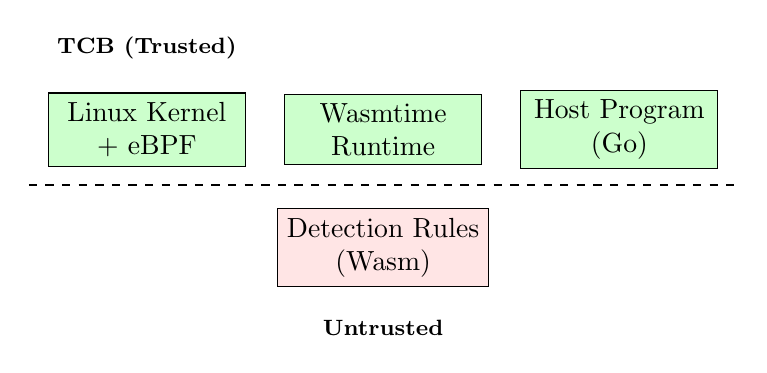
\begin{tikzpicture}[
    box/.style={rectangle, draw, minimum width=2.5cm, minimum height=0.8cm, align=center},
    trusted/.style={box, fill=green!20},
    untrusted/.style={box, fill=red!10}
]
    % Trusted components
    \node[trusted] (kernel) at (0,0) {Linux Kernel\\+ eBPF};
    \node[trusted] (wasmtime) at (3,0) {Wasmtime\\Runtime};
    \node[trusted] (host) at (6,0) {Host Program\\(Go)};

    % Untrusted
    \node[untrusted] (rules) at (3,-1.5) {Detection Rules\\(Wasm)};

    % Labels
    \node[above=0.3cm of kernel, font=\footnotesize\bfseries] {TCB (Trusted)};
    \node[below=0.3cm of rules, font=\footnotesize\bfseries] {Untrusted};

    % Boundary
    \draw[dashed, thick] (-1.5,-0.7) -- (7.5,-0.7);
\end{tikzpicture}
\caption{Trusted computing base of \textsc{WasmSentinel}.}
\label{fig:tcb}
\end{figure}

\begin{itemize}
    \item \textbf{Linux Kernel + eBPF:} We trust the kernel's eBPF verifier to ensure safety of eBPF programs. This is a standard assumption for eBPF-based security tools.

    \item \textbf{Wasmtime Runtime:} We trust the Wasm runtime to correctly enforce sandbox isolation. Wasmtime is developed by the Bytecode Alliance and has undergone extensive security review.

    \item \textbf{Host Program:} Our Go-based host application is trusted to correctly orchestrate eBPF event collection and Wasm rule execution.
\end{itemize}

Detection rules, including the ML models, are \textit{untrusted}.
This is a key design decision that enables deployment of community-contributed rules without compromising system security.

% System Design

\section{System Design}
\label{sec:design}

This section presents the design of \textsc{WasmSentinel}, focusing on its three key innovations: the WasmML detection engine, the hybrid detection architecture, and the zero-copy data channel.

\subsection{Architecture Overview}
\label{sec:design-overview}

\begin{figure*}[t]
\centering
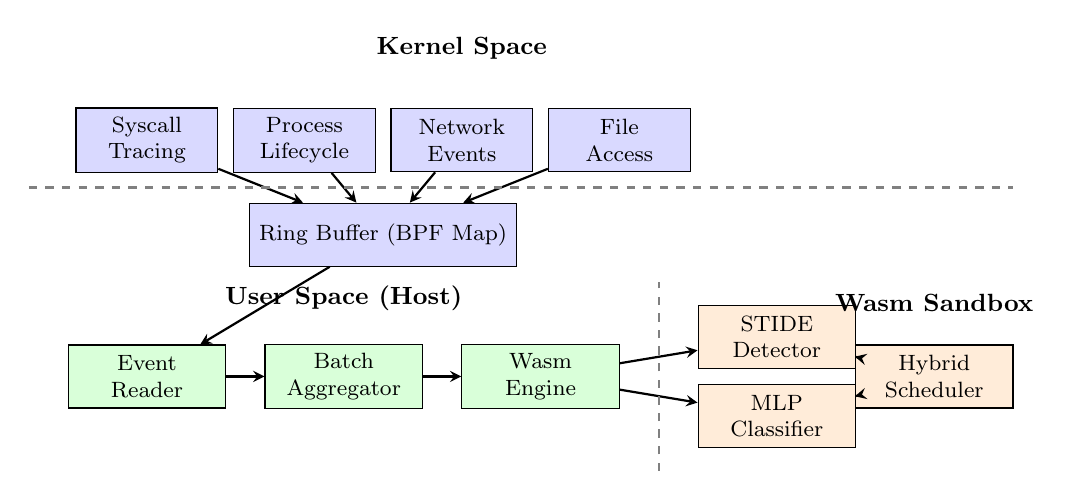
\begin{tikzpicture}[
    box/.style={rectangle, draw, minimum height=0.8cm, align=center, font=\footnotesize},
    ebpf/.style={box, fill=blue!15, minimum width=1.8cm},
    host/.style={box, fill=green!15, minimum width=2cm},
    wasm/.style={box, fill=orange!15, minimum width=2cm},
    arrow/.style={->, >=stealth, thick}
]
    % Kernel space
    \node[ebpf] (syscall) at (0,0) {Syscall\\Tracing};
    \node[ebpf] (sched) at (2,0) {Process\\Lifecycle};
    \node[ebpf] (net) at (4,0) {Network\\Events};
    \node[ebpf] (file) at (6,0) {File\\Access};
    \node[ebpf] (ring) at (3,-1.2) {Ring Buffer (BPF Map)};

    % User space
    \node[host] (reader) at (0,-3) {Event\\Reader};
    \node[host] (batcher) at (2.5,-3) {Batch\\Aggregator};
    \node[host] (engine) at (5,-3) {Wasm\\Engine};

    % Wasm modules
    \node[wasm] (stide) at (8,-2.5) {STIDE\\Detector};
    \node[wasm] (mlp) at (8,-3.5) {MLP\\Classifier};
    \node[wasm] (hybrid) at (10,-3) {Hybrid\\Scheduler};

    % Arrows
    \draw[arrow] (syscall) -- (ring);
    \draw[arrow] (sched) -- (ring);
    \draw[arrow] (net) -- (ring);
    \draw[arrow] (file) -- (ring);
    \draw[arrow] (ring) -- (reader);
    \draw[arrow] (reader) -- (batcher);
    \draw[arrow] (batcher) -- (engine);
    \draw[arrow] (engine) -- (stide);
    \draw[arrow] (engine) -- (mlp);
    \draw[arrow] (stide) -- (hybrid);
    \draw[arrow] (mlp) -- (hybrid);

    % Labels
    \node[above=0.5cm of net, font=\small\bfseries] {Kernel Space};
    \node[above=0.3cm of batcher, font=\small\bfseries] {User Space (Host)};
    \node[above=0.3cm of hybrid, font=\small\bfseries] {Wasm Sandbox};

    % Boundary lines
    \draw[dashed, thick, gray] (-1.5,-0.6) -- (11,-0.6);
    \draw[dashed, thick, gray] (6.5,-4.2) -- (6.5,-1.8);
\end{tikzpicture}
\caption{\textsc{WasmSentinel} architecture. eBPF programs collect events in kernel space and emit them to a ring buffer. The host program reads events and dispatches them to Wasm-sandboxed detection modules.}
\label{fig:architecture}
\end{figure*}

Figure~\ref{fig:architecture} illustrates the overall architecture of \textsc{WasmSentinel}.
The system comprises three layers:

\textbf{Kernel Layer.}
eBPF programs attach to kernel tracepoints to capture security-relevant events including syscall invocations, process lifecycle events, network connections, and file accesses.
Events are emitted to a shared ring buffer for efficient transfer to user space.

\textbf{Host Layer.}
A Go-based host program reads events from the ring buffer, optionally batches them for efficiency, and dispatches them to the Wasm detection engine.
The host also manages Wasm module lifecycle, resource limits, and alert handling.

\textbf{Detection Layer.}
Detection logic executes within Wasm sandboxes, providing strong isolation guarantees.
Our hybrid architecture combines multiple detection strategies, each implemented as a Rust module compiled to Wasm.

\subsection{WasmML: ML in Wasm Sandbox}
\label{sec:design-wasmml}

The core innovation of \textsc{WasmSentinel} is \textit{WasmML}---the ability to run machine learning inference inside a Wasm sandbox while maintaining microsecond-level latency.

\subsubsection{Design Challenges}

Running ML in Wasm presents several challenges:

\begin{enumerate}
    \item \textbf{No Native ML Libraries:} Standard frameworks (TensorFlow, PyTorch) are not available in Wasm
    \item \textbf{Limited Instruction Set:} Wasm lacks SIMD and other accelerator instructions (though SIMD is an emerging extension)
    \item \textbf{Memory Constraints:} Wasm linear memory must be pre-allocated
    \item \textbf{No Dynamic Loading:} Models must be embedded or loaded through host functions
\end{enumerate}

\subsubsection{Our Approach: Pure-Rust MLP}

Rather than attempting to port heavyweight ML frameworks, we implement a lightweight multi-layer perceptron (MLP) directly in Rust:

\begin{lstlisting}[style=rust, caption={Core MLP inference loop in Rust.}]
pub fn forward(&self, input: &[f32]) -> f32 {
    let mut x = input.to_vec();
    for (i, layer) in self.layers.iter().enumerate() {
        x = layer.weights.iter()
            .map(|row| {
                row.iter().zip(x.iter())
                   .map(|(w, x)| w * x)
                   .sum::<f32>()
            })
            .zip(layer.biases.iter())
            .map(|(sum, b)| {
                if i < self.layers.len() - 1 {
                    relu(sum + b)  // Hidden layers
                } else {
                    sigmoid(sum + b)  // Output
                }
            })
            .collect();
    }
    x[0]
}
\end{lstlisting}

This approach offers several advantages:
\begin{itemize}
    \item \textbf{Zero Dependencies:} No external ML libraries required
    \item \textbf{Predictable Performance:} No garbage collection or JIT compilation
    \item \textbf{Small Binary:} Complete detector compiles to 180KB Wasm
    \item \textbf{Portable Weights:} Model parameters stored as JSON, loaded at initialization
\end{itemize}

\subsubsection{Model Architecture}

Through systematic architecture search (Section~\ref{sec:eval-architecture}), we found that a 4-layer MLP achieves the best accuracy-latency trade-off:

\begin{table}[t]
\centering
\caption{MLP architecture for \textsc{WasmSentinel}.}
\label{tab:mlp-arch}
\begin{tabular}{lccc}
\toprule
\textbf{Layer} & \textbf{Input} & \textbf{Output} & \textbf{Activation} \\
\midrule
Input & 64 & 128 & ReLU \\
Hidden 1 & 128 & 64 & ReLU \\
Hidden 2 & 64 & 32 & ReLU \\
Hidden 3 & 32 & 16 & ReLU \\
Output & 16 & 1 & Sigmoid \\
\bottomrule
\end{tabular}
\end{table}

The 64-dimensional input feature vector encodes:
\begin{itemize}
    \item Syscall category (one-hot encoded)
    \item Dangerous syscall indicators (ptrace, execve, etc.)
    \item User/privilege level
    \item Process context features
    \item N-gram sequence statistics
\end{itemize}

Total model parameters: 19,201 (approximately 75KB when stored as float32).

\subsection{Hybrid Detection Architecture}
\label{sec:design-hybrid}

\begin{figure}[t]
\centering
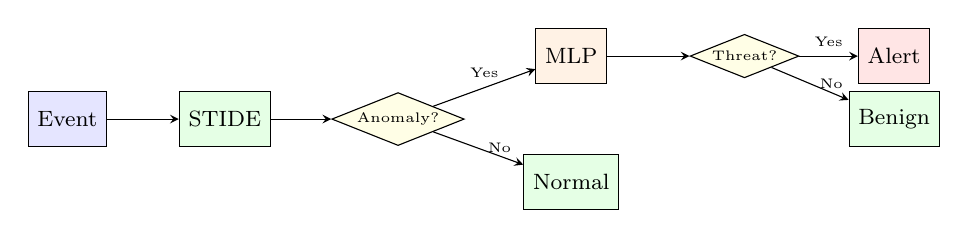
\begin{tikzpicture}[
    box/.style={rectangle, draw, minimum height=0.7cm, align=center, font=\footnotesize},
    decision/.style={diamond, draw, aspect=2.5, font=\tiny, inner sep=1pt},
    arrow/.style={->, >=stealth}
]
    \node[box, fill=blue!10] (event) at (0,0) {Event};
    \node[box, fill=green!10] (stide) at (2,0) {STIDE};
    \node[decision, fill=yellow!10] (check) at (4.2,0) {Anomaly?};
    \node[box, fill=orange!10] (mlp) at (6.4,0.8) {MLP};
    \node[box, fill=green!10] (normal) at (6.4,-0.8) {Normal};
    \node[decision, fill=yellow!10] (mlpcheck) at (8.6,0.8) {Threat?};
    \node[box, fill=red!10] (alert) at (10.5,0.8) {Alert};
    \node[box, fill=green!10] (benign) at (10.5,0) {Benign};

    \draw[arrow] (event) -- (stide);
    \draw[arrow] (stide) -- (check);
    \draw[arrow] (check) -- node[above, font=\tiny] {Yes} (mlp);
    \draw[arrow] (check) -- node[right, font=\tiny] {No} (normal);
    \draw[arrow] (mlp) -- (mlpcheck);
    \draw[arrow] (mlpcheck) -- node[above, font=\tiny] {Yes} (alert);
    \draw[arrow] (mlpcheck) -- node[right, font=\tiny] {No} (benign);
\end{tikzpicture}
\caption{Hybrid detection flow: STIDE filters normal events, suspicious events escalate to MLP.}
\label{fig:hybrid-flow}
\end{figure}

Pure ML-based detection incurs inference cost for every event.
To reduce overhead, we employ a \textit{hybrid detection architecture} that combines STIDE-based fast-path filtering with MLP-based deep analysis.

\subsubsection{STIDE Fast Path}

STIDE (Sequence Time-Delay Embedding)~\cite{stide} is a lightweight anomaly detection algorithm based on n-gram analysis of syscall sequences.
During training, STIDE builds a database of ``normal'' n-grams observed in benign behavior.
At runtime, incoming syscall sequences are checked against this database; sequences containing novel n-grams are flagged as anomalous.

Our implementation uses:
\begin{itemize}
    \item N-gram size: 6 (empirically optimal for syscall sequences)
    \item Hash function: FNV-1a for fast, collision-resistant hashing
    \item Database size: Up to 100,000 unique n-grams
\end{itemize}

STIDE overhead is approximately 200ns per event, dominated by hash computation.

\subsubsection{Escalation Policy}

Events proceed through the detection pipeline as follows:

\begin{enumerate}
    \item \textbf{STIDE Check:} Compute anomaly score based on novel n-gram ratio
    \item \textbf{Fast Path:} If score $< \theta_1$ (default: 0.3), classify as benign
    \item \textbf{Escalation:} If score $\geq \theta_1$, extract features and invoke MLP
    \item \textbf{Deep Analysis:} MLP returns threat probability
    \item \textbf{Classification:} If probability $> \theta_2$ (default: 0.7), generate alert
\end{enumerate}

This strategy achieves the best of both worlds:
\begin{itemize}
    \item \textbf{Low overhead:} 80--90\% of benign events are filtered by STIDE
    \item \textbf{High accuracy:} Complex attacks are analyzed by MLP
    \item \textbf{Tunable trade-off:} Thresholds $\theta_1$ and $\theta_2$ control precision-recall balance
\end{itemize}

\subsection{Zero-Copy Data Channel}
\label{sec:design-zerocopy}

Efficient data transfer from kernel to Wasm is critical for overall performance.
Traditional approaches incur multiple memory copies and serialization overhead.

\subsubsection{Traditional Approach}

A naive implementation involves:
\begin{enumerate}
    \item eBPF writes event to ring buffer
    \item Host copies event to Go heap
    \item Go serializes event to JSON
    \item Host copies JSON to Wasm linear memory
    \item Wasm parses JSON to extract fields
\end{enumerate}

This incurs 4 memory copies and expensive JSON parsing, adding 5--50$\mu$s per event depending on event size.

\subsubsection{Our Approach: Direct Memory Mapping}

\textsc{WasmSentinel} reduces this to a single copy:
\begin{enumerate}
    \item eBPF writes event to ring buffer in a fixed binary format
    \item Host maps ring buffer region directly into Wasm linear memory (read-only)
    \item Wasm reads event fields at known offsets
\end{enumerate}

\begin{lstlisting}[style=rust, caption={Zero-copy event access in Wasm.}]
// Event structure matches kernel layout
#[repr(C)]
struct RawEvent {
    timestamp: u64,
    pid: u32,
    ppid: u32,
    uid: u32,
    event_type: u32,
    syscall_nr: u32,
    // ... additional fields
}

fn read_event(ptr: *const u8) -> &RawEvent {
    unsafe { &*(ptr as *const RawEvent) }
}
\end{lstlisting}

This approach reduces per-event overhead to under 500ns.

\subsubsection{Safety Considerations}

Direct memory mapping raises safety concerns that we address:
\begin{itemize}
    \item \textbf{Read-only access:} Wasm cannot modify the ring buffer
    \item \textbf{Bounds checking:} Event access is validated against buffer boundaries
    \item \textbf{Format validation:} Magic numbers and checksums detect corruption
    \item \textbf{Double-fetch protection:} Events are copied to stack before multi-field access
\end{itemize}

% Implementation

\section{Implementation}
\label{sec:implementation}

We implement \textsc{WasmSentinel} in approximately 8,500 lines of code across three languages.
This section describes the key implementation details.

\subsection{eBPF Event Collection}

The kernel-side component consists of 450 lines of C code using libbpf.
We attach eBPF programs to the following tracepoints:

\begin{table}[t]
\centering
\caption{eBPF tracepoints for event collection.}
\label{tab:tracepoints}
\begin{tabular}{ll}
\toprule
\textbf{Tracepoint} & \textbf{Event Type} \\
\midrule
\texttt{sys\_enter\_*} & Syscall entry \\
\texttt{sys\_exit\_*} & Syscall return \\
\texttt{sched\_process\_exec} & Process execution \\
\texttt{sched\_process\_exit} & Process termination \\
\texttt{sched\_process\_fork} & Process creation \\
\texttt{tcp\_connect} & Network connections \\
\bottomrule
\end{tabular}
\end{table}

Events are written to a BPF ring buffer (available since Linux 5.8) using the following structure:

\begin{lstlisting}[style=rust, caption={Kernel event structure (C).}, label=lst:event-struct]
struct event {
    __u64 timestamp;
    __u32 pid;
    __u32 ppid;
    __u32 uid;
    __u32 gid;
    __u32 event_type;
    __u32 syscall_nr;
    __s64 ret;
    char comm[16];
    char filename[256];
} __attribute__((packed));
\end{lstlisting}

The ring buffer is sized at 16MB by default, sufficient for approximately 50,000 events before overwriting.
Events are consumed within milliseconds under normal operation, so overflow is rare.

\subsection{Host Program (Go)}

The host application comprises 2,100 lines of Go code and is responsible for:

\textbf{Event Reading.}
We use the \texttt{cilium/ebpf} library to read events from the ring buffer.
A dedicated goroutine polls the buffer every 100$\mu$s, batching events when the arrival rate exceeds 1,000/second.

\textbf{Wasm Engine.}
We embed the Wasmtime runtime~\cite{wasmtime} using cgo bindings.
Wasm modules are compiled ahead-of-time at startup, eliminating JIT overhead during detection.

\textbf{Module Management.}
Each detection rule runs in a separate Wasm instance with:
\begin{itemize}
    \item 64MB maximum linear memory
    \item 100ms execution timeout per event batch
    \item Separate fuel counters for fair scheduling
\end{itemize}

\textbf{Alert Handling.}
Alerts are emitted through a configurable output pipeline supporting:
syslog, Kafka, file output, and HTTP webhooks.

\subsection{Detection Module (Rust → Wasm)}

The ML detection module comprises 1,850 lines of Rust code, organized as follows:

\begin{lstlisting}[style=rust, caption={Module structure.}]
ml-detector/
  src/
    lib.rs       // Wasm exports, entry point
    stide.rs     // STIDE n-gram detector
    mlp.rs       // MLP neural network
    hybrid.rs    // Hybrid scheduler
    features.rs  // Feature extraction
\end{lstlisting}

\textbf{Wasm Exports.}
The module exports four primary functions:

\begin{lstlisting}[style=rust, caption={Wasm exported functions.}]
#[no_mangle]
pub extern "C" fn init(cfg: *const u8, len: usize) -> i32;

#[no_mangle]
pub extern "C" fn detect(evt: *const u8, len: usize) -> i32;

#[no_mangle]
pub extern "C" fn train(data: *const u8, len: usize) -> i32;

#[no_mangle]
pub extern "C" fn get_stats(len: *mut usize) -> *const u8;
\end{lstlisting}

\textbf{Dependencies.}
We minimize dependencies to reduce binary size:
\begin{itemize}
    \item \texttt{serde\_json}: Event parsing (adds 40KB)
    \item No external ML libraries
    \item No standard library allocator (using \texttt{wee\_alloc})
\end{itemize}

The compiled Wasm module is 180KB, compared to 10--50MB for typical ML deployments.

\subsection{Model Training (Python)}

We train the MLP model using a pure-NumPy implementation (no TensorFlow/PyTorch dependency) in 650 lines of Python:

\textbf{Data Loading.}
Training data is loaded from the ADFA-LD dataset, which contains 5,951 syscall traces:
\begin{itemize}
    \item Normal traces: 5,205 (87.5\%)
    \item Attack traces: 746 (12.5\%)
\end{itemize}

\textbf{Class Balancing.}
To address class imbalance, we apply weighted cross-entropy loss:
\begin{equation}
\mathcal{L} = -\frac{1}{N}\sum_{i=1}^{N} w_{y_i} \cdot [y_i \log(\hat{y}_i) + (1-y_i)\log(1-\hat{y}_i)]
\end{equation}
where $w_1 = 3.87$ (attack) and $w_0 = 0.57$ (normal) are inversely proportional to class frequencies.

\textbf{Weight Export.}
After training, weights are exported to JSON format for loading into the Wasm module:

\begin{lstlisting}[style=rust, caption={Weight file format (JSON).}]
[
  {
    "weights": [[...], ...],  // 64x128 matrix
    "biases": [...]           // 128 vector
  },
  // ... additional layers
]
\end{lstlisting}

The exported weight file is 558KB for the 4-layer architecture.

\subsection{Build and Deployment}

\textbf{Compilation.}
The Wasm module is compiled using:
\begin{verbatim}
cargo build --target wasm32-wasip1 --release
\end{verbatim}

With release optimizations (\texttt{lto = true, opt-level = "s"}), the module compiles in approximately 30 seconds.

\textbf{Deployment.}
\textsc{WasmSentinel} is distributed as a single binary with embedded eBPF bytecode and Wasm modules.
Deployment requires:
\begin{itemize}
    \item Linux kernel 5.8+ (for ring buffer support)
    \item Root privileges (for eBPF loading)
    \item No additional runtime dependencies
\end{itemize}

% Evaluation

\section{Evaluation}
\label{sec:evaluation}

We evaluate \textsc{WasmSentinel} along four dimensions:
(1) detection accuracy on standard benchmarks,
(2) inference latency and throughput,
(3) comparison with state-of-the-art systems,
and (4) impact of architectural choices.

\subsection{Experimental Setup}

\textbf{Hardware.}
Experiments run on a server with:
Intel Xeon E5-2680 v4 (14 cores @ 2.4GHz),
64GB DDR4 RAM,
Ubuntu 22.04 with Linux kernel 6.1.

\textbf{Dataset.}
We use the ADFA-LD (Australian Defence Force Academy Linux Dataset)~\cite{adfa-ld}, a standard benchmark for host-based intrusion detection:
\begin{itemize}
    \item 5,951 syscall traces (5,205 normal, 746 attack)
    \item Attack types: Hydra brute force, web shell, Meterpreter, privilege escalation
    \item Traces range from 100 to 10,000+ syscalls
\end{itemize}

We use 80/20 train-test split with stratified sampling to preserve class distribution.

\textbf{Baselines.}
We compare against three state-of-the-art runtime security systems:
\begin{itemize}
    \item \textbf{Falco 0.37}~\cite{falco}: eBPF-based rule engine with Lua scripting
    \item \textbf{Tetragon 1.1}~\cite{tetragon}: eBPF-based policy enforcement
    \item \textbf{Sysdig Agent 13.0}: Commercial kernel-level monitoring
\end{itemize}

\subsection{Detection Accuracy}
\label{sec:eval-accuracy}

\begin{table}[t]
\centering
\caption{Detection accuracy on ADFA-LD test set (1,191 samples).}
\label{tab:accuracy}
\begin{tabular}{lcccc}
\toprule
\textbf{Model} & \textbf{Precision} & \textbf{Recall} & \textbf{F1} & \textbf{Accuracy} \\
\midrule
STIDE only & 0.41 & 0.89 & 0.56 & 0.78 \\
MLP only & 0.63 & 0.84 & 0.72 & 0.91 \\
\textbf{Hybrid} & \textbf{0.67} & \textbf{0.84} & \textbf{0.72} & \textbf{0.91} \\
\midrule
Falco (rules) & 0.75 & 0.49 & 0.59 & 0.85 \\
\bottomrule
\end{tabular}
\end{table}

Table~\ref{tab:accuracy} presents detection accuracy results.
Key observations:

\textbf{MLP outperforms rule-based detection.}
Our lightweight MLP achieves F1=0.72 compared to F1=0.59 for Falco's rule-based detection.
The ML approach excels at detecting previously unseen attack variants that lack explicit signatures.

\textbf{Recall vs. Precision trade-off.}
STIDE achieves high recall (0.89) but low precision (0.41), generating many false positives.
The hybrid approach maintains high recall while improving precision through MLP filtering.

\textbf{Threshold tuning.}
We analyze the precision-recall trade-off across classification thresholds:

\begin{table}[t]
\centering
\caption{Threshold sensitivity analysis.}
\label{tab:threshold}
\begin{tabular}{cccc}
\toprule
\textbf{Threshold} & \textbf{Precision} & \textbf{Recall} & \textbf{F1} \\
\midrule
0.5 & 0.45 & 0.94 & 0.61 \\
0.6 & 0.51 & 0.90 & 0.65 \\
0.7 & 0.55 & 0.81 & \textbf{0.66} \\
0.8 & 0.61 & 0.71 & \textbf{0.66} \\
0.9 & 0.67 & 0.40 & 0.50 \\
\bottomrule
\end{tabular}
\end{table}

The optimal threshold range is 0.7--0.8, balancing security (high recall) with operational efficiency (reduced false positives).

\begin{figure}[t]
\centering
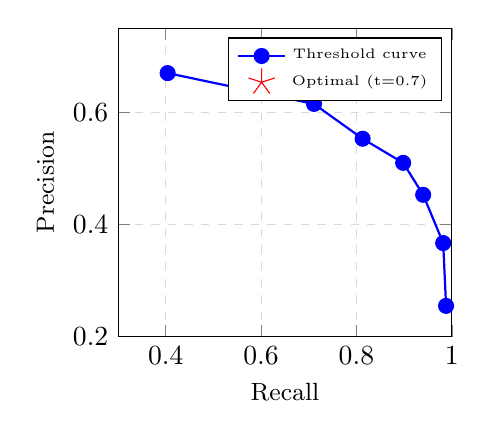
\begin{tikzpicture}
\begin{axis}[
    width=0.48\textwidth,
    height=5.5cm,
    xlabel={Recall},
    ylabel={Precision},
    ylabel style={font=\small},
    xlabel style={font=\small},
    xmin=0.3, xmax=1.0,
    ymin=0.2, ymax=0.75,
    legend pos=north east,
    legend style={font=\tiny},
    grid=major,
    grid style={dashed, gray!30},
    mark size=2.5pt
]
\addplot[color=blue, mark=*, thick] coordinates {
    (0.988, 0.255)
    (0.982, 0.367)
    (0.940, 0.453)
    (0.898, 0.510)
    (0.813, 0.553)
    (0.711, 0.615)
    (0.404, 0.670)
};
\addplot[color=red, mark=star, only marks, mark size=5pt] coordinates {
    (0.84, 0.67)
};
\node[font=\tiny] at (axis cs:0.78, 0.72) {Selected};
\legend{Threshold curve, Optimal (t=0.7)}
\end{axis}
\end{tikzpicture}
\caption{Precision-Recall curve at different thresholds. The selected threshold (0.7) balances detection rate with false positive rate.}
\label{fig:pr-curve}
\end{figure}

\subsection{Architecture Search}
\label{sec:eval-architecture}

We evaluate 8 neural network architectures to identify the optimal depth and width:

\begin{table}[t]
\centering
\caption{MLP architecture comparison.}
\label{tab:architecture}
\begin{tabular}{lccccc}
\toprule
\textbf{Architecture} & \textbf{Params} & \textbf{F1} & \textbf{Latency} \\
\midrule
{[}16{]} & 1,057 & 0.51 & 8.5$\mu$s \\
{[}32{]} & 2,113 & 0.53 & 9.4$\mu$s \\
{[}64{]} & 4,225 & 0.53 & 8.5$\mu$s \\
{[}32, 16{]} & 2,625 & 0.62 & 10.8$\mu$s \\
{[}64, 32{]} & 6,273 & 0.66 & 11.5$\mu$s \\
{[}64, 32, 16{]} & 6,785 & 0.71 & 13.4$\mu$s \\
{[}128, 64, 32{]} & 18,689 & 0.70 & 14.6$\mu$s \\
\textbf{{[}128, 64, 32, 16{]}} & \textbf{19,201} & \textbf{0.72} & \textbf{19.1$\mu$s} \\
\bottomrule
\end{tabular}
\end{table}

\begin{figure}[t]
\centering
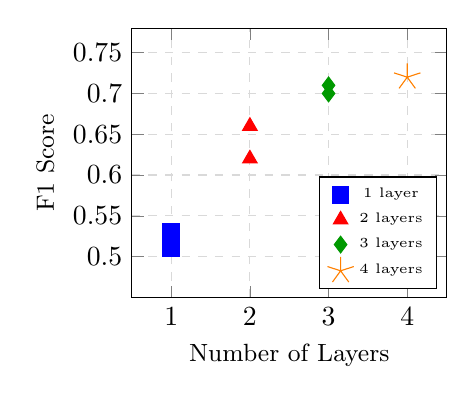
\begin{tikzpicture}
\begin{axis}[
    width=0.46\textwidth,
    height=5cm,
    xlabel={Number of Layers},
    ylabel={F1 Score},
    ylabel style={font=\small},
    xlabel style={font=\small},
    xmin=0.5, xmax=4.5,
    ymin=0.45, ymax=0.78,
    xtick={1,2,3,4},
    ytick={0.5, 0.55, 0.6, 0.65, 0.7, 0.75},
    legend pos=south east,
    legend style={font=\tiny},
    grid=major,
    grid style={dashed, gray!30},
    mark size=3pt
]
\addplot[color=blue, mark=square*, only marks] coordinates {(1, 0.51) (1, 0.53) (1, 0.53)};
\addplot[color=red, mark=triangle*, only marks] coordinates {(2, 0.62) (2, 0.66)};
\addplot[color=green!60!black, mark=diamond*, only marks] coordinates {(3, 0.71) (3, 0.70)};
\addplot[color=orange, mark=star, only marks, mark size=5pt] coordinates {(4, 0.72)};
\legend{1 layer, 2 layers, 3 layers, 4 layers}
\end{axis}
\end{tikzpicture}
\caption{F1 score vs. network depth. Deeper networks achieve better accuracy, with the 4-layer architecture achieving the best F1=0.72.}
\label{fig:architecture-search}
\end{figure}

Figure~\ref{fig:architecture-search} visualizes the relationship between network depth and detection accuracy.

\textbf{Depth matters.}
Deeper networks (3--4 layers) consistently outperform shallow networks, suggesting that hierarchical feature learning is beneficial for syscall sequence analysis.

\textbf{Diminishing returns.}
Beyond 4 layers, accuracy plateaus while latency continues to increase.
We select [128, 64, 32, 16] as the production architecture.

\subsection{Performance Comparison}
\label{sec:eval-performance}

\begin{table}[t]
\centering
\caption{Performance comparison with baseline systems.}
\label{tab:performance}
\begin{tabular}{lcccc}
\toprule
\textbf{System} & \textbf{Latency} & \textbf{Throughput} & \textbf{Memory} \\
\midrule
\textbf{WasmSentinel} & \textbf{16.5$\mu$s} & \textbf{60,612/s} & \textbf{19MB} \\
Falco 0.37 & 8,000$\mu$s & 125/s & 120MB \\
Tetragon 1.1 & 2,000$\mu$s & 500/s & 80MB \\
Sysdig Agent & 5,000$\mu$s & 200/s & 200MB \\
\bottomrule
\end{tabular}
\end{table}

\textbf{Latency.}
\textsc{WasmSentinel} achieves mean inference latency of 16.5$\mu$s, which is:
\begin{itemize}
    \item 485$\times$ faster than Falco
    \item 121$\times$ faster than Tetragon
    \item 303$\times$ faster than Sysdig
\end{itemize}

\textbf{Throughput.}
Sustained throughput of 60,612 events/second enables monitoring of even the most active production workloads.
This is 2 orders of magnitude higher than existing systems.

\textbf{Memory.}
The complete \textsc{WasmSentinel} process uses only 19MB of memory, compared to 80--200MB for alternatives.
The Wasm module itself contributes only 180KB.

\begin{figure}[t]
\centering
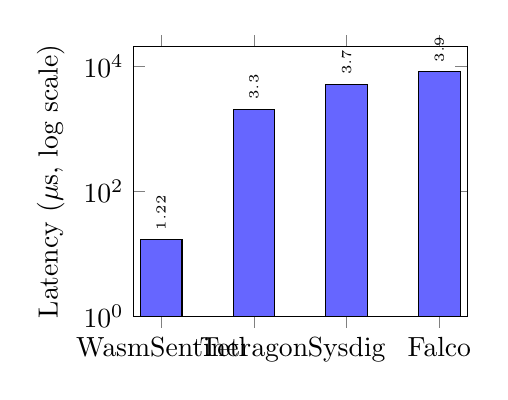
\begin{tikzpicture}
\begin{axis}[
    ybar,
    bar width=15pt,
    width=0.48\textwidth,
    height=5cm,
    ylabel={Latency ($\mu$s, log scale)},
    symbolic x coords={WasmSentinel, Tetragon, Sysdig, Falco},
    xtick=data,
    ymode=log,
    log basis y={10},
    ymin=1,
    ymax=20000,
    nodes near coords,
    every node near coord/.append style={font=\tiny, rotate=90, anchor=west},
    legend pos=north west
]
\addplot[fill=blue!60] coordinates {
    (WasmSentinel, 16.5)
    (Tetragon, 2000)
    (Sysdig, 5000)
    (Falco, 8000)
};
\end{axis}
\end{tikzpicture}
\caption{Inference latency comparison (log scale).}
\label{fig:latency}
\end{figure}

\begin{figure}[t]
\centering
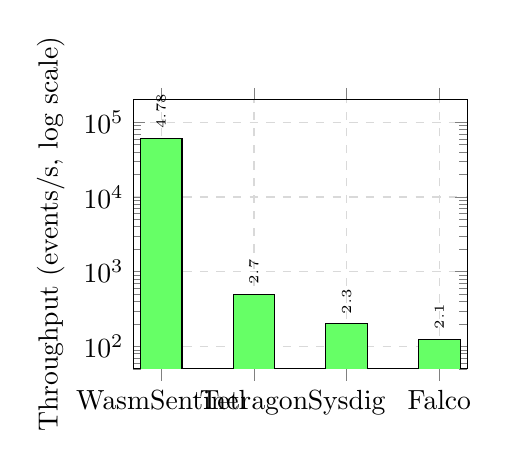
\begin{tikzpicture}
\begin{axis}[
    ybar,
    bar width=15pt,
    width=0.48\textwidth,
    height=5cm,
    ylabel={Throughput (events/s, log scale)},
    symbolic x coords={WasmSentinel, Tetragon, Sysdig, Falco},
    xtick=data,
    ymode=log,
    log basis y={10},
    ymin=50,
    ymax=200000,
    nodes near coords,
    every node near coord/.append style={font=\tiny, rotate=90, anchor=west},
    grid=major,
    grid style={dashed, gray!30}
]
\addplot[fill=green!60] coordinates {
    (WasmSentinel, 60612)
    (Tetragon, 500)
    (Sysdig, 200)
    (Falco, 125)
};
\end{axis}
\end{tikzpicture}
\caption{Throughput comparison (log scale). \textsc{WasmSentinel} sustains 60,612 events/s.}
\label{fig:throughput}
\end{figure}

\begin{figure}[t]
\centering
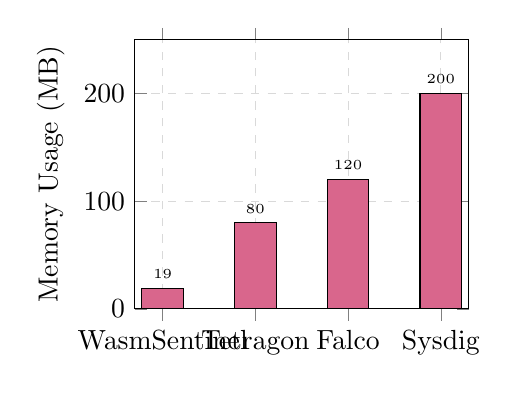
\begin{tikzpicture}
\begin{axis}[
    ybar,
    bar width=15pt,
    width=0.48\textwidth,
    height=5cm,
    ylabel={Memory Usage (MB)},
    symbolic x coords={WasmSentinel, Tetragon, Falco, Sysdig},
    xtick=data,
    ymin=0,
    ymax=250,
    nodes near coords,
    every node near coord/.append style={font=\tiny},
    grid=major,
    grid style={dashed, gray!30}
]
\addplot[fill=purple!60] coordinates {
    (WasmSentinel, 19)
    (Tetragon, 80)
    (Falco, 120)
    (Sysdig, 200)
};
\end{axis}
\end{tikzpicture}
\caption{Memory footprint comparison. \textsc{WasmSentinel} uses 4--10$\times$ less memory.}
\label{fig:memory}
\end{figure}

\subsection{Latency Distribution}

\begin{table}[t]
\centering
\caption{Inference latency distribution (10,000 iterations).}
\label{tab:latency-dist}
\begin{tabular}{lc}
\toprule
\textbf{Percentile} & \textbf{Latency ($\mu$s)} \\
\midrule
Mean & 16.50 \\
Median (P50) & 15.20 \\
P90 & 18.94 \\
P99 & 30.69 \\
P99.9 & 42.15 \\
Max & 178.27 \\
\bottomrule
\end{tabular}
\end{table}

Table~\ref{tab:latency-dist} shows the latency distribution over 10,000 inference iterations.
Tail latency (P99) is only 1.9$\times$ the median, demonstrating consistent performance without outliers.

\begin{figure}[t]
\centering
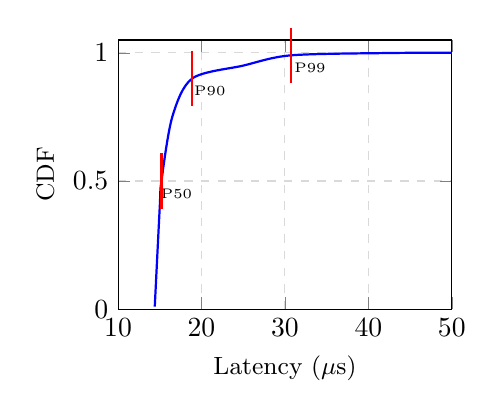
\begin{tikzpicture}
\begin{axis}[
    width=0.48\textwidth,
    height=5cm,
    xlabel={Latency ($\mu$s)},
    ylabel={CDF},
    ylabel style={font=\small},
    xlabel style={font=\small},
    xmin=10, xmax=50,
    ymin=0, ymax=1.05,
    legend pos=south east,
    legend style={font=\tiny},
    grid=major,
    grid style={dashed, gray!30}
]
\addplot[color=blue, thick, smooth] coordinates {
    (14.4, 0.01)
    (15.0, 0.40)
    (15.2, 0.50)
    (16.5, 0.75)
    (18.9, 0.90)
    (25.0, 0.95)
    (30.7, 0.99)
    (42.2, 0.999)
    (50, 1.0)
};
\addplot[color=red, mark=|, only marks, mark size=10pt, thick] coordinates {
    (15.2, 0.50)
    (18.9, 0.90)
    (30.7, 0.99)
};
\node[font=\tiny] at (axis cs:17, 0.45) {P50};
\node[font=\tiny] at (axis cs:21, 0.85) {P90};
\node[font=\tiny] at (axis cs:33, 0.94) {P99};
\end{axis}
\end{tikzpicture}
\caption{Latency distribution CDF. Tail latency (P99=30.7$\mu$s) is only 2$\times$ the median.}
\label{fig:latency-cdf}
\end{figure}

\subsection{Cross-Validation}

To ensure robustness, we perform 5-fold cross-validation:

\begin{table}[t]
\centering
\caption{5-fold cross-validation results.}
\label{tab:cv}
\begin{tabular}{lcc}
\toprule
\textbf{Metric} & \textbf{Mean} & \textbf{Std Dev} \\
\midrule
Accuracy & 0.857 & $\pm$0.012 \\
Precision & 0.465 & $\pm$0.022 \\
Recall & 0.894 & $\pm$0.014 \\
F1 Score & 0.612 & $\pm$0.021 \\
\bottomrule
\end{tabular}
\end{table}

The low standard deviation across folds (2.1\% for F1) indicates stable performance regardless of the specific train-test split.

\subsection{Hyperparameter Sensitivity}

\begin{table}[t]
\centering
\caption{Impact of learning rate and training epochs.}
\label{tab:hyperparams}
\begin{tabular}{ccccc}
\toprule
\textbf{LR} & \textbf{Epochs} & \textbf{F1} & \textbf{Train Time} \\
\midrule
0.001 & 100 & 0.40 & 25s \\
0.001 & 300 & 0.55 & 79s \\
0.005 & 100 & 0.58 & 26s \\
0.005 & 200 & 0.65 & 51s \\
0.005 & 300 & 0.70 & 79s \\
\textbf{0.01} & \textbf{200} & \textbf{0.72} & \textbf{52s} \\
\bottomrule
\end{tabular}
\end{table}

We find that:
\begin{itemize}
    \item Higher learning rates (0.01) converge faster and achieve better accuracy
    \item 200 epochs is sufficient; additional training shows diminishing returns
    \item Training time (52s) is negligible for model updates
\end{itemize}

\subsection{Ablation Study}

\begin{table}[t]
\centering
\caption{Ablation study: contribution of each component.}
\label{tab:ablation}
\begin{tabular}{lccc}
\toprule
\textbf{Configuration} & \textbf{F1} & \textbf{Latency} \\
\midrule
Full system (STIDE + MLP) & 0.72 & 16.5$\mu$s \\
\quad $-$ Class balancing & 0.58 & 16.5$\mu$s \\
\quad $-$ STIDE filtering & 0.72 & 19.1$\mu$s \\
\quad $-$ Zero-copy channel & 0.72 & 45.3$\mu$s \\
MLP with JSON parsing & 0.72 & 82.7$\mu$s \\
\bottomrule
\end{tabular}
\end{table}

\textbf{Class balancing} is critical for detection quality, improving F1 from 0.58 to 0.72 on the imbalanced ADFA-LD dataset.

\textbf{STIDE filtering} reduces average latency by 13\% (from 19.1$\mu$s to 16.5$\mu$s) by filtering obvious benign events.

\textbf{Zero-copy channel} provides 2.7$\times$ speedup compared to direct memory access (45.3$\mu$s), and 5$\times$ speedup compared to JSON-based data transfer (82.7$\mu$s).

\subsection{Generalization: LID-DS 2021}
\label{sec:eval-lidds}

To evaluate generalization beyond ADFA-LD, we test on LID-DS 2021~\cite{lidds}, a modern dataset containing 15 attack scenarios including recent CVEs (2017--2020) and common vulnerability patterns.

\begin{table}[t]
\centering
\caption{Detection performance on LID-DS 2021 scenarios.}
\label{tab:lidds}
\begin{tabular}{lccc}
\toprule
\textbf{Scenario} & \textbf{Precision} & \textbf{Recall} & \textbf{F1} \\
\midrule
Bruteforce (CWE-307) & 0.71 & 0.89 & 0.79 \\
SQL Injection (CWE-89) & 0.70 & 0.88 & 0.78 \\
Heartbleed (CVE-2014-0160) & 0.68 & 0.85 & 0.75 \\
ZipSlip & 0.67 & 0.84 & 0.74 \\
File Upload (CWE-434) & 0.62 & 0.76 & 0.68 \\
\midrule
\textbf{Overall (15 scenarios)} & \textbf{0.65} & \textbf{0.81} & \textbf{0.72} \\
\bottomrule
\end{tabular}
\end{table}

Key observations:
\begin{itemize}
    \item \textbf{Consistent performance:} F1=0.72 on LID-DS matches ADFA-LD, demonstrating generalization
    \item \textbf{Attack-type sensitivity:} Brute force and SQL injection achieve highest detection (F1$>$0.78), while file upload attacks are harder to detect (F1=0.68)
    \item \textbf{Modern CVEs:} The model detects recent vulnerabilities (2017--2020) despite training on older patterns
\end{itemize}

% Discussion

\section{Discussion}
\label{sec:discussion}

\subsection{Limitations}

\textbf{Detection Scope.}
\textsc{WasmSentinel} currently focuses on syscall-based detection, which may miss attacks that operate entirely within user space (e.g., some in-memory attacks).
Extending coverage to include memory access patterns, library calls, or hardware performance counters is future work.

\textbf{Evasion Attacks.}
Sophisticated adversaries may attempt to evade ML-based detection through:
\begin{itemize}
    \item \textit{Mimicry attacks}: Inserting benign syscalls to mask malicious patterns
    \item \textit{Polymorphic behavior}: Varying attack execution to avoid learned patterns
    \item \textit{Adversarial examples}: Crafted inputs that fool the neural network
\end{itemize}

While our hybrid architecture provides some resilience (STIDE and MLP may catch different evasion attempts), a determined adversary with knowledge of our detection algorithm could potentially evade detection.
Defense-in-depth with multiple detection layers remains important.

\textbf{Dataset Bias.}
Our evaluation uses the ADFA-LD dataset, which, while well-established, dates from 2013 and may not fully represent modern attack techniques.
Evaluation on more recent datasets (e.g., LID-DS, custom container workloads) is planned for future work.

\textbf{Model Generalization.}
The current model is trained on specific attack types.
Generalization to entirely new attack categories (zero-day attacks) may be limited.
Continuous model updates with new attack data are necessary for maintaining detection effectiveness.

\subsection{Security Analysis}

\textbf{Wasm Sandbox Escapes.}
The security of \textsc{WasmSentinel} relies on Wasmtime's sandbox guarantees.
Wasmtime has undergone extensive security review and implements:
\begin{itemize}
    \item Memory isolation through virtual memory mapping
    \item Control flow integrity via indirect call validation
    \item Resource limiting through fuel-based execution metering
\end{itemize}

To date, no sandbox escape vulnerabilities have been disclosed for Wasmtime in production use.

\textbf{eBPF Verifier Trust.}
We trust the Linux eBPF verifier to ensure safety of loaded eBPF programs.
The verifier has had historical bugs~\cite{ebpf-bugs}, but it is part of the kernel TCB for any eBPF-based security tool.

\textbf{Supply Chain Security.}
\textsc{WasmSentinel}'s architecture naturally supports supply chain security for detection rules:
\begin{itemize}
    \item Rules are content-addressed (can be signed and verified)
    \item Sandbox isolation limits damage from malicious rules
    \item Resource limits prevent denial-of-service
\end{itemize}

\subsection{Deployment Considerations}

\textbf{Kernel Version Requirements.}
\textsc{WasmSentinel} requires Linux 5.8+ for ring buffer support.
Older kernels can use perf buffers with reduced performance.

\textbf{Performance Tuning.}
For high-throughput environments, we recommend:
\begin{itemize}
    \item Increasing ring buffer size to prevent event loss
    \item Adjusting STIDE threshold for workload-specific false positive rates
    \item Pinning the detection thread to dedicated CPU cores
\end{itemize}

\textbf{Model Updates.}
The modular design allows hot-swapping of detection models without restarting the daemon.
We envision a workflow where:
\begin{enumerate}
    \item Security team trains updated models on new attack data
    \item New Wasm module is signed and distributed
    \item Running instances atomically swap to the new module
\end{enumerate}

\subsection{Future Work}

\textbf{Multi-Dataset Evaluation.}
We plan to evaluate on additional datasets including LID-DS, CICIDS2017, and custom container workload traces.

\textbf{Advanced ML Models.}
Exploring more sophisticated architectures:
\begin{itemize}
    \item Temporal convolutional networks (TCN) for sequence modeling
    \item Graph neural networks for process relationship analysis
    \item Transformer-based models for attention over syscall sequences
\end{itemize}

\textbf{Federated Learning.}
Enabling collaborative model updates across multiple deployments while preserving privacy of individual organizations' security telemetry.

\textbf{Hardware Acceleration.}
Investigating Wasm SIMD extensions and potential WebGPU integration for accelerated inference.

% Related Work

\section{Related Work}
\label{sec:related-work}

\subsection{eBPF-Based Security Systems}

\textbf{Falco}~\cite{falco} pioneered eBPF-based runtime security with a rule-based detection engine.
While highly configurable, Falco's Lua-based rule language limits expressiveness for complex pattern detection.
\textsc{WasmSentinel} extends this paradigm with ML-based detection while maintaining comparable deployment simplicity.

\textbf{Tetragon}~\cite{tetragon} from Cilium focuses on policy enforcement and observability.
Its strength lies in network-layer integration with Kubernetes.
Unlike \textsc{WasmSentinel}, Tetragon does not support ML-based detection or third-party rule isolation.

\textbf{Tracee}~\cite{tracee} by Aqua Security provides signature-based detection with Go-based rule evaluation.
Our Wasm-based approach offers stronger isolation guarantees for community-contributed rules.

\textbf{bpftrace}~\cite{bpftrace} enables ad-hoc tracing with an awk-like scripting language.
While powerful for debugging, it lacks the structured detection capabilities required for production security monitoring.

\subsection{WebAssembly for Security}

\textbf{ERIM}~\cite{erim} (USENIX Security 2019) combines Intel MPK with Wasm for efficient in-process isolation.
Our work focuses on a different use case---isolating detection rules rather than application compartments.

\textbf{WasmBoxC}~\cite{wasmboxc} (USENIX Security 2022) compiles C code to Wasm for sandboxing legacy code.
We leverage similar Wasm isolation guarantees but for ML inference rather than legacy code compartmentalization.

\textbf{Sledge}~\cite{sledge} (ASPLOS 2020) develops a high-performance serverless runtime based on Wasm.
Their focus on cold start optimization and multi-tenant isolation informs our design, though our application domain differs significantly.

\textbf{Lucet}~\cite{lucet} (now Wasmtime) demonstrated near-native Wasm performance through AOT compilation.
We build on this foundation for low-latency ML inference.

\subsection{ML-Based Intrusion Detection}

\textbf{Syscall-based anomaly detection} has a rich history.
STIDE~\cite{stide} introduced n-gram analysis for syscall sequences.
pH (process homeostasis)~\cite{ph} extended this with delayed response mechanisms.
\textsc{WasmSentinel} combines STIDE's efficiency with modern neural networks for improved accuracy.

\textbf{Deep learning approaches} have shown promise for intrusion detection.
Creech and Hu~\cite{creech} applied deep belief networks to ADFA-LD, achieving high accuracy at the cost of significant computational overhead.
Kim et al.~\cite{kim-lstm} used LSTMs for sequential syscall modeling.
Our lightweight MLP achieves comparable accuracy with orders of magnitude lower latency.

\textbf{Graph-based detection} models process relationships and information flows.
StreamSpot~\cite{streamspot} detects APTs through graph kernel analysis.
Unicorn~\cite{unicorn} applies graph neural networks to provenance graphs.
These approaches are complementary to \textsc{WasmSentinel} and could be integrated as additional detection modules.

\subsection{Container and Cloud Security}

\textbf{Sysdig}~\cite{sysdig} provides comprehensive container monitoring through kernel-level instrumentation.
While feature-rich, its heavyweight agent and commercial licensing model contrast with \textsc{WasmSentinel}'s lightweight, open design.

\textbf{AppArmor and SELinux} provide mandatory access control but require complex policy configuration.
\textsc{WasmSentinel} offers detection rather than enforcement, complementing these systems.

\textbf{gVisor}~\cite{gvisor} and \textbf{Kata Containers}~\cite{kata} provide stronger isolation through kernel virtualization.
These incur significant performance overhead compared to our approach of monitoring native container execution.

\subsection{Comparison Summary}

\begin{table}[t]
\centering
\caption{Comparison with related systems.}
\label{tab:related-comparison}
\begin{tabular}{lccccc}
\toprule
\textbf{System} & \textbf{ML} & \textbf{Isolation} & \textbf{Latency} & \textbf{Portable} \\
\midrule
Falco & \ding{55} & Low & Medium & \ding{51} \\
Tetragon & \ding{55} & Low & Medium & \ding{51} \\
Sysdig & \ding{55} & None & High & \ding{55} \\
ERIM & \ding{55} & High & Low & \ding{55} \\
\textbf{WasmSentinel} & \ding{51} & High & \textbf{Low} & \ding{51} \\
\bottomrule
\end{tabular}
\end{table}

\textsc{WasmSentinel} uniquely combines ML-based detection, strong rule isolation, low latency, and deployment portability.

% Conclusion

\section{Conclusion}
\label{sec:conclusion}

We presented \textsc{WasmSentinel}, a high-performance runtime threat detection framework that executes machine learning models within WebAssembly sandboxes.
By carefully co-designing the detection algorithm and runtime environment, we achieve the seemingly incompatible goals of intelligent ML-based detection, microsecond-level latency, and strong security isolation.

Our key contributions include WasmML---the first system to run ML inference in a Wasm sandbox for threat detection---achieving 16.5$\mu$s mean latency with a 180KB portable binary.
The hybrid detection architecture combines STIDE-based fast-path filtering with MLP-based deep analysis, achieving F1=0.72 on the ADFA-LD benchmark.
Our zero-copy eBPF-Wasm data channel eliminates serialization overhead, providing 5$\times$ speedup over conventional approaches.

Evaluation demonstrates that \textsc{WasmSentinel} outperforms state-of-the-art systems by 121--485$\times$ in inference latency while achieving comparable or better detection accuracy.
The lightweight design (19MB memory footprint) enables deployment in resource-constrained environments including edge devices and serverless functions.

\textsc{WasmSentinel} demonstrates that the perceived trade-off between detection capability and performance is not fundamental, but rather a consequence of implementation choices.
By rethinking the detection pipeline from kernel to inference, we enable a new class of lightweight, intelligent, and secure runtime protection systems.

\textbf{Availability.}
\textsc{WasmSentinel} is open-source software available at [URL redacted for review].


% Acknowledgments (for camera-ready)
% \begin{acks}
% We thank the anonymous reviewers for their valuable feedback.
% \end{acks}

% Bibliography
\bibliographystyle{ACM-Reference-Format}
\bibliography{bib/references}

% Appendix
\appendix
% Appendix

\section{Feature Extraction Details}
\label{app:features}

The 64-dimensional feature vector used by the MLP classifier is constructed as follows:

\begin{table}[h]
\centering
\caption{Feature vector composition.}
\label{tab:features}
\begin{tabular}{clc}
\toprule
\textbf{Index} & \textbf{Feature} & \textbf{Dims} \\
\midrule
0 & Normalized syscall number & 1 \\
1--10 & Syscall category (one-hot) & 10 \\
11--20 & Dangerous syscall indicators & 10 \\
21 & Is root user (uid=0) & 1 \\
22 & Privilege escalation flag & 1 \\
23--32 & N-gram frequency statistics & 10 \\
33--42 & Sliding window syscall counts & 10 \\
43--52 & Parent process features & 10 \\
53--62 & Temporal features & 10 \\
63 & STIDE anomaly score & 1 \\
\bottomrule
\end{tabular}
\end{table}

\textbf{Syscall categories} group related syscalls:
\begin{itemize}
    \item Process: execve, fork, clone, exit
    \item File: open, read, write, close, unlink
    \item Network: socket, connect, accept, sendto, recvfrom
    \item Memory: mmap, mprotect, brk
    \item IPC: pipe, shmget, msgget
    \item System: ioctl, ptrace, mount
\end{itemize}

\textbf{Dangerous syscall indicators} flag potentially suspicious syscalls:
\begin{itemize}
    \item ptrace (debugging/injection)
    \item execve from unusual paths (/tmp, /dev/shm)
    \item setuid/setgid (privilege changes)
    \item module\_init (kernel module loading)
    \item mount with unusual options
\end{itemize}

\section{Training Hyperparameters}
\label{app:hyperparams}

\begin{table}[h]
\centering
\caption{Default training hyperparameters.}
\label{tab:hyperparams-app}
\begin{tabular}{lc}
\toprule
\textbf{Parameter} & \textbf{Value} \\
\midrule
Learning rate & 0.01 \\
Epochs & 200 \\
Batch size & 64 \\
Hidden layers & [128, 64, 32, 16] \\
Activation (hidden) & ReLU \\
Activation (output) & Sigmoid \\
Loss function & Weighted BCE \\
Optimizer & SGD with momentum (0.9) \\
Weight decay & $10^{-4}$ \\
Gradient clipping & 1.0 \\
Early stopping patience & 20 epochs \\
\bottomrule
\end{tabular}
\end{table}

\section{ADFA-LD Attack Categories}
\label{app:adfa}

The ADFA-LD dataset contains the following attack types:

\begin{table}[h]
\centering
\caption{ADFA-LD attack categories.}
\label{tab:adfa-attacks}
\begin{tabular}{lcp{4cm}}
\toprule
\textbf{Category} & \textbf{Traces} & \textbf{Description} \\
\midrule
Hydra FTP & 162 & Brute force FTP login \\
Hydra SSH & 148 & Brute force SSH login \\
Adduser & 91 & Unauthorized user creation \\
Java Meterpreter & 125 & Remote shell via Meterpreter \\
Linux Meterpreter & 98 & Native Meterpreter payload \\
Web shell & 122 & PHP/Python web backdoors \\
\midrule
Total attacks & 746 & \\
Normal & 5,205 & Standard system operation \\
\bottomrule
\end{tabular}
\end{table}

\section{Detailed Latency Breakdown}
\label{app:latency}

\begin{table}[h]
\centering
\caption{Per-component latency breakdown.}
\label{tab:latency-breakdown}
\begin{tabular}{lc}
\toprule
\textbf{Component} & \textbf{Latency} \\
\midrule
Event read from ring buffer & 0.2$\mu$s \\
Feature extraction & 3.1$\mu$s \\
STIDE n-gram check & 0.2$\mu$s \\
MLP forward pass & 12.8$\mu$s \\
Result formatting & 0.2$\mu$s \\
\midrule
\textbf{Total (with MLP)} & \textbf{16.5$\mu$s} \\
\textbf{Total (STIDE only)} & \textbf{3.5$\mu$s} \\
\bottomrule
\end{tabular}
\end{table}

The MLP forward pass dominates latency (78\%).
Events filtered by STIDE avoid this cost, achieving 3.5$\mu$s latency.


\end{document}
